\documentclass[10pt,letterpaper]{article}
\usepackage{authblk}
\usepackage{hyperref}
\usepackage{cogsci}
\usepackage{pslatex}
\usepackage{apacite}
\usepackage{physics}
\usepackage{graphicx}
\usepackage{amssymb}
\usepackage{amsmath}
\usepackage{caption}
\usepackage{subcaption}

\usepackage{booktabs}
\hyphenpenalty=9999
\usepackage{xcolor}
\usepackage{url}
\definecolor{Blue}{RGB}{50,50,200}
\definecolor{Green}{RGB}{50,200,50}
\definecolor{Red}{RGB}{200,50,50}
\newcommand{\hh}[1]{\textcolor{Blue}{@hh: #1}}
\newcommand{\cl}[1]{\textcolor{Green}{@cl: #1}}

% model colors
\definecolor{VGG-19}{RGB}{245, 126, 32}
\definecolor{Inception-V3}{RGB}{174,199,232}
\definecolor{ResNet-50}{RGB}{158, 208, 137}
\definecolor{ViT-B}{RGB}{246,181,209}
\definecolor{Swin-B}{RGB}{213, 41, 40}
\definecolor{MLPMixer-B}{RGB}{246,150,150}
\definecolor{MoCo-v2}{RGB}{140, 87, 76}
\definecolor{MoCo-v3}{RGB}{140, 87, 76}
\definecolor{DINO}{RGB}{245, 126, 32}
\definecolor{CLIP}{RGB}{252, 186, 120}
\definecolor{Noisy Student}{RGB}{146,104,172}
\definecolor{SWSL}{RGB}{45,160,72}
\definecolor{MAE}{RGB}{215,121,177}


\DeclareMathOperator*{\argmin}{arg\,min} % thin space, limits underneath in displays
\DeclareMathOperator*{\argmax}{arg\,max} % thin space, limits underneath in displays

\title{Evaluating machine comprehension of sketch meaning at different levels of abstraction}
 
\cogscifinalcopy % Uncomment this line for the final submission 

\author[1]{\bf Kushin Mukherjee}
\author[2]{\bf Holly Huey}
\author[2]{\bf Xuanchen Lu}
\author[3]{\bf Yael Vinker}
\author[2]{\bf Rio Aguina-Kang}
\author[5]{\bf Ariel Shamir}
\author[2,4]{\bf Judith E. Fan}

\affil[1]{University of Wisconsin-Madison, Madison, WI, United States}
\affil[2]{University of California, San Diego, CA, United States}
\affil[3]{Tel-Aviv University, Tel-Aviv, Israel}
\affil[4]{Stanford University, Stanford, CA, United States}
\affil[5]{Reichman University, Herzliya, Israel}

% \author{{\large \bf Holly Huey (hhuey@ucsd.edu)} \\
%   \AND {\large \bf Judith E. Fan (jefan@ucsd.edu)} \\
%   Department of Psychology, University of California, San Diego \\
%   9500 Gilman Dr., La Jolla, CA 92093 USA}
\begin{document}
% \makeatletter
% \let\@oldmaketitle\@maketitle% Store \@maketitle
% \renewcommand{\@maketitle}{\@oldmaketitle% 

% \makeatother
\maketitle
\begin{abstract}

People can reliably understand images that vary in visual abstraction---from detailed illustrations to schematic icons. 
To what degree are current vision algorithms robust to such variation when attributing meaning to abstract images? 
We first obtained $>90K$ human-generated sketches produced under different time limits (4s, 8s, 16s, 32s; $N$=5,563 participants) and AI-generated sketches \cite{vinker2022clipasso} produced under different ink limits (4, 8, 16, 32 strokes) of 2,048 real-world object concepts spanning 128 categories from the THINGS dataset \cite{hebart2019things}.
We then evaluated how well 12 state-of-the-art vision algorithms could (1) predict which concept each sketch was intended to convey and (2) match human performance and response patterns when presented with the same sketches.
We found that models achieving generally higher recognition accuracy also tracked human error patterns better, although there remains a sizable gap between human and machine sketch understanding.  
We also found that, on average, different models expressed similar uncertainty about sketches of the same concept across different levels of abstraction.
We hope that public release of this dataset and evaluation protocol will lead to algorithms that display more human-like visual abstraction. 
% Together, these findings suggest promising avenues for building better models of human visual abstraction. 

\textbf{Keywords:} 
concepts; drawing; perception; computer vision; benchmark
\end{abstract}

\section{Introduction}

Humans can use pictures to convey what they perceive and know at varying levels of abstraction---from detailed illustrations to simple sketches.
Indeed, the ability to abstract away from the particulars of any given experience to highlight the most important elements is inherent in the act of creating any effective visualization \cite{viola2017pondering, chen2020foundations,mccloud1998understanding, mi2009abstraction, nan2011conjoining}.
Line drawings present an especially important case study in the capacity for visual abstraction, as demonstrated by the Spanish artist Pablo Picasso in his renown work, \textit{The Bull} (1945), which contains 11 lithographs of bulls, each successively more abstract than the last (Fig.~\ref{fig:bulls}).
Despite striking variation in their degree of fidelity to the real world, understanding what even the most abstract of these images represent feels effortless for most human viewers.

Such variation is manifest in works of art, but is also pervasive across many domains of human activity. 
% , line drawings present an important case study in visual abstraction given their versatility and ubiquity in human culture.
Not only do most cultures produce drawings \cite{gombrich1995story}, the ability to produce line drawings that capture key aspects of the real world also emerges early in development \cite{karmiloff1990constraints, dillon2021rooms, long2021parallel}, and the visual properties of these drawings have been linked to children's developing conceptual knowledge \cite{tversky1989parts,huey2022developmental}. 
Additionally, failures to produce and understand pictures of objects at different levels of abstraction is associated with semantic dementia \cite{bozeat2003duck, rogers2007object}, suggesting links between a robust capacity for visual abstraction and the functional organization of semantic knowledge in the brain. 
What are the core visual computations that support this ability to grasp the meaning of pictures across so many different levels of visual abstraction? 

% of the world—objects, scenes, and events—at varying levels of abstraction. 
% Humans have the ability to visually communicate their knowledge of the world—objects, scenes, and events—at varying levels of abstraction. 
% could both depict scenes with incredible detail and attention towards preserving the likeness to the real world, as well as depict concepts like ``dog'' with only a single stroke by omitting much of the information that would help the sketch share a visual resemblance to a real dog. 
% The relevance and necessity to abstract visually across many different levels arises across many instances of visual communication.
% In certain contexts, a faithful and detailed depiction might be what is required, such as when an architect conveys detailed schematics to an engineer \cite{suwa1997architects} or when a zoologist creates scientific illustrations of a new animal species \cite{baigrie1996picturing}. 
% However in other contexts, such as when there exists established social conventions or when resources are limited (e.g., time), simpler depictions can be used to efficiently denote objects \cite{fan2020pragmatic, garrod2007foundations, hawkins2021visual}. 
% Amongst these cases, one tool for visualization that might showcase the greatest variability in visual abstraction while being widely pervasive are line drawings \cite{sayim2011line}.

\begin{figure}[t]
    \centering
    \includegraphics[width=0.7\linewidth]{figures/picasso_bulls.jpg}
    \caption{Pablo Picasso. \textit{The Bull}, 1945.}
    \label{fig:bulls}
    \vspace{-2em}
\end{figure}


% both kinds of depictions can be understood and recognized by those who view them. 

% This notion that knowledge can be flexibly expressed and understood at many such levels of abstraction, while raised in prior work  \cite{viola2017pondering, chen2020foundations,mccloud1998understanding}, has evaded a generalized formal account. 
% As a consequence, it has remained unclear to what degree modern vision algorithms can support varied representations of the same underlying concept spanning multiple degrees of abstraction.

% While many might agree that knowledge can be flexibly expressed and comprehended at such different levels of abstraction, a formal account of visual abstraction has remained largely absent in the .
% For example, in the domain of sketching, a sketcher can choose to produce a highly-detailed realistic drawing or a simplified stylized drawing. 
% From an observer's perspective, the former might be evocative of a specific flower, such as a rose, the latter might convey the general concept of 'flower'. 

% Thus, drawings are ubiquitous in culture and development, a window into learned semantics, and exhibit variation in perceived abstractness.
% These properties make drawings of real-world objects a uniquely well-suited vehicle for understanding visual abstraction and developing common protocols for measurement of this construct across humans and machines mirroring similar efforts in cognitive science and AI \cite{bear2021physion}.

The past several years have seen remarkable progress in uncovering the mechanisms by which the human visual system achieves a robust understanding of the visual world \cite{yamins2014performance, kriegeskorte2015deep, zhuang2021unsupervised, konkle2022self}. 
These mechanistic models now often take the form of trainable neural networks combining several architectural motifs inspired by the primate ventral visual stream 
% including its hierarchical organization and local circuit properties 
\cite{gross1972visual,goodale1992separate,malach2002topography,hung2005fast}. %--- though not in all cases \cite{dosovitskiy2020image}.
These advances have also recently been applied to the problem of sketch understanding, revealing both the value of these approaches for learning general-purpose perceptual representations to model human visual abstraction \cite{fan2018common, yu2017sketch, kubilius2016deep}, as well as persistent challenges in achieving the capacity for robust understanding of visual inputs that vary in their degree of visual abstraction \cite{baker2018abstract, singer2022photos, fan2020pragmatic}.

\begin{figure*}
    \centering
    \includegraphics[width=.93\linewidth]{figures/VAB_methods_4.pdf}
    \vspace{-0.5em}
    \caption{Human sketchers \& CLIPasso generated $>90K$ sketches under different production constraints: drawing time \& number of strokes, respectively.}
    \label{fig:example_gallery}
    \vspace{-1.5em}
\end{figure*}

Despite these great strides in the development of high-performing vision models, it remains unclear to what degree the \textit{specific} models that have been proposed so far achieve human-like understanding of such a broad range of visual inputs, from natural images to human-generated drawings and symbols.
Evaluating this question has been especially challenging given that, while there are several widely used benchmark sketch datasets \cite{eitz2012sketch, jongejan2017quick, sangkloy2016sketchy}, none of them systematically vary the degree of detail, a salient axis differentiating depictions of specific instances from more abstract illustrations. %, in the sketches they contain. 

In this paper, we take two major steps towards closing this gap: 
(1) we develop a large dataset containing human ($N$=5,563 participants) and AI-generated sketches varying in detail, for a representatively wide variety of visual object concepts varying in their degree of abstraction; 
and (2) we systematically evaluate how well 12 diverse state-of-the-art vision models, varying in their architectures and training methods, represent semantic information in these sketches by benchmarking their recognition performance against human behavior. 
We build on a growing body of research leveraging a global image dataset generated by the THINGS initiative \cite{hebart2019things} by sampling 2,048 real-world objects spanning 128 concepts as referents for drawings in our dataset.
% We leverage the drawings to investigate which axes of variation among vision models might be most salient for human-like understanding of drawings.
Our main goals were to test the consistency between models and humans in their ability to recognize the concepts depicted in our sketch dataset, as well as the alignment between distributions of human-generated soft labels ($N$=3,190 participants)  and distributions underlying model classification performance \cite{collins2022eliciting,peterson2019human}.
% Moreover, although we evaluate a specific set of models in the current paper, we intend our approach to serve as a general evaluation framework that may be used to for measure sensitivity to visual abstraction in any model.
% , which constitute a meaningful new dimension along which all future vision model can be evaluated along.
Taken together, our work aims to contribute an informative benchmark of human and machine generated sketches spanning varying multiple levels of abstraction. 
We hope that publicly releasing our datasets and proposed methods for investigating sketch understanding will generate opportunities for future research avenues towards building better computational models of human visual abstraction.
% \textit{first,} we collected a large number of human-generated sketches produced under different time limits (4s, 8s, 16s, 32s; $N$=5,563 participants) and AI-generated sketches \cite{vinker2022clipasso} produced under different ink limits (8, 16, 32 strokes) of 2,048 real-world objects spanning 128 categories from the THINGS dataset \cite{hebart2019things}. \textit{Second,} we conducted a systematic evaluation of how well several state-of-the-art vision algorithms, varying in their architecture and training, represent the meaning of these sketches, without additional training.
% Taken together, our study aims to provide a useful benchmark dataset and framework for probing sketch understanding in machines, and point to promising avenues for building better computational models of human visual abstraction in future work.

% A critical requirement for such efforts is a dataset depicting a sufficiently diverse set of objects at varying levels of abstraction. Using a time-restricted drawing paradigm, we present such a dataset of human-produced drawings depicting 2048 exemplars of 128 unique concepts. We also leverage recent advances in machine sketch-generation \cite{vinker2022clipasso} to create machine-produced drawings at varying levels of abstraction. Next, we evaluate a suite of modern vision algorithms which vary in their architectures, training paradigms, and training datasets, in their sensitivity to variations in abstraction. While we find many dimensions of variance across latent neural representations in their ability to capture variations in abstractness, we show that convolutional neural networks and models trained on semi-supervised learning methods are among the most sensitive to these variations.

% This serves as an important first step towards the systematic study of visual abstraction in both humans and machines.

% This body of work from diverse areas of cognitive science lends support to the notion that


% \subsection{Computational models of vision}
% Deep learning models, including convolutional neural networks (see \citeNP{li2021survey} for a review) and vision transformers \cite{dosovitskiy2020image}, are often considered the best contemporary models of human visual perception \cite{kriegeskorte2015deep,kubilius2019brain,lindsay2021deep} even in the domain of drawings \cite{fan2018common}. But how sensitive are these algorithms to semantic abstraction of the kinds described earlier? Here, we first collect a dataset of human and machine sketches .... spanning different levels of visual abstraction. Next, we evaluate representations extracted from a suite of vision models at various stages of processing (early, intermediate, and late) to measure their ability to represent visual concepts at different levels of abstraction using novel formalizations of visual abstraction.

% \section{Sketching at varying levels of abstraction}

\section{Method}
% The current paper has two key aims: 
% (1) to develop a large dataset containing human and AI-generated sketches that vary in their degree of abstraction, for a wide variety of visual object concepts; 
% and (2) to evaluate how well various state-of-the-art vision models represent semantic information about these sketches, including information about the target object at the category and exemplar levels, without additional training. 
Our first goal was to generate two parallel large-scale drawing datasets spanning varying levels of abstraction: one produced by humans under varying time limits (4s, 8s, 16s, and 32s), and the other by automatic machine generation varying in the number of strokes per drawing (4, 8, 16, and 32 strokes), using CLIPasso \cite{vinker2022clipasso} (see Fig. ~\ref{fig:example_gallery} for example sketches).   
Next, to estimate recognizability of the drawings in both datasets, we conducted an independent recognition study in which participants provided one or more labels for a representative sample of human and machine drawings.

% In order to generate human drawings that spanned a variety of abstractions, we adapted a time-restricted drawing task used in work by \citeauthor{berger2013style} (2013) and asked people to produce drawings of objects in 4, 8, 16, and 32 seconds.
% Here we hypothesized that under time constraints, people would produce drawings that are not only less detailed but also more evocative of the general concept they were asked to draw, relative to a specific instance of that concept.


\subsubsection{Stimuli}
% THINGS database
To generate a diverse large-scale stimulus set of object concepts, we systematically sampled 128 concepts from the database of the THINGS initiative, a global database of 1,854 object concepts (e.g., ``lion'', ``banjo'', ``car'') and naturalistic object images aimed at developing a multi-varied cognitive neuroscience and behavioral metrics on a shared set of objects \cite{hebart2019things}. 
Building on prior work by \citeauthor{yang2021visual} (2021) investigating visual abstraction across different contexts, we selected concepts based on similar parameters spanning four main axes of variation: familiarity, artificiality, animacy, and size. 
Within each object concept, we randomly sampled 16 object images. 
Our final stimuli set included 2,048 object images that were used as referents for the human and machine sketching tasks.

\subsection{Human Sketch Production Task} 
\subsubsection{Participants} 
5,563 participants (2,870 male; $M_{age}$ = 36.7 years) were recruited from Prolific to produce a series of sketches on a web-based drawing platform. 
% Data collection stopped when 10 sketches had been generated for each of the 2,048 object images.
We excluded 104 data sessions from participants, who experienced technical difficulties.
In this and all subsequent tasks, participants provided informed consent in accordance with the UC San Diego IRB.

\subsubsection{Procedure}
 We randomly assigned participants to one of four conditions, each varying in the amount of time that they were permitted to use to generate their drawings: 4, 8, 16, or 32 seconds (Fig.~\ref{fig:example_gallery}, \textit{left}). 
Each participant produced 16 drawings of different object concepts.
During each trial, participants were presented with an object label, a corresponding object photograph (500px x 500px) to give participants a concrete example of what the object looks like, and a drawing canvas (500px x 500px). 
They were instructed to produce a drawing of the general concept represented by the label, and that, they should not include details specific to the instance of the object in the provided photograph. 
Next to the canvas, participants were given a countdown timer indicating how many seconds they had left to produce their drawing. 
% To ensure that participants were prepared to draw given the short duration of each condition, a reminder about the drawing duration was interleaved between drawing trials that also provided participants the opportunity to take a short break and to indicate when they were ready to start the next trial. 
A trial ended when the timer ran out or when the participant pressed the ``Continue'' button if they finished their sketch with time remaining, although they were instructed to try to use as much time as they needed to accurately represent the prompted concept.
Participants were were instructed not to include any background context (e.g., grass in a drawing of a ``horse''), arrows, or text.
Participants also completed a practice trial before the test drawing trials to familiarize themselves to the drawing platform, including the ability to undo their most recent stroke or completely clear their canvas if needed. 

\begin{figure}[]
    \centering
    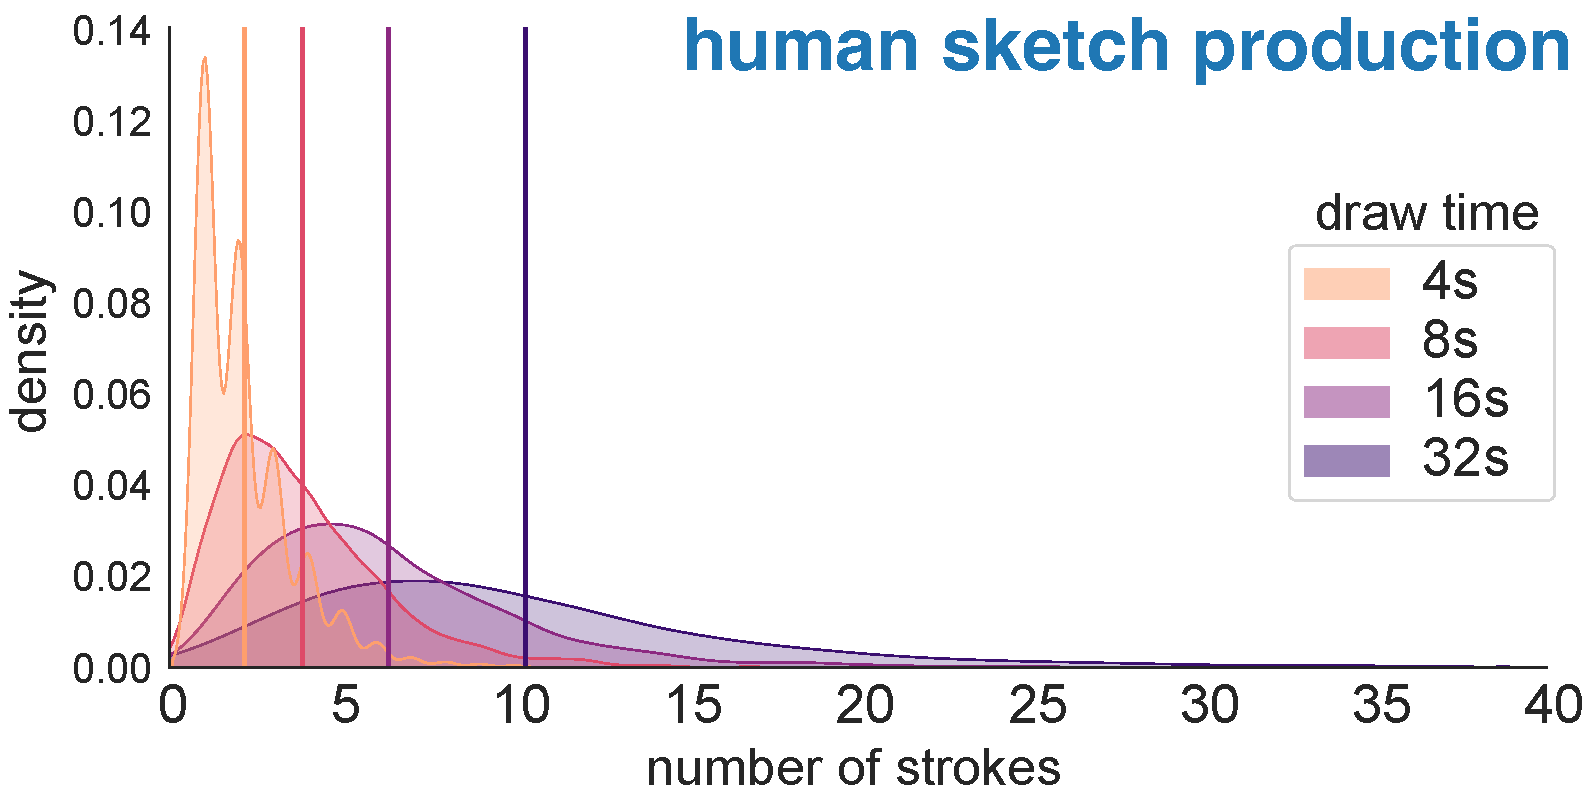
\includegraphics[width=.95\linewidth]{figures/VAB_stroke_complexity_v2.pdf}
        \vspace{-1em}
    \caption{Stroke distributions. Vertical lines indicate means.}
    \label{fig:stroke_counts}
    \vspace{-1.5em}
\end{figure}

\subsection{Machine Sketch Generation}
We leveraged CLIPasso \cite{vinker2022clipasso}, a recently developed sketch generation algorithm, to also generate sketches of the same 2,048 object images. 
CLIPasso generates sketches by optimizing the parameters of a set of curves (strokes) to align to a latent representation of an image of an object computed by CLIP \cite{radford2021learning}, a neural network model trained on a large corpus of text-image pairs.
For each image, we generated sketches at four levels of abstraction using 4, 8, 16, and 32 strokes (Fig.~\ref{fig:example_gallery}, \textit{right}) as an approximately parallel manipulation of the time-restriction paradigm of our human production task.

\subsection{Human Sketch Recognition Task}
We next aimed to develop a recognizability baseline for each sketch to compare to model classification performance. 
To accomplish this, we designed a web-based recognition study to crowdsource object labels associated with each sketch in order to capture its perceived meaning.
Critically, because sketches often capture a range of semantic meaning that can bring to mind many possible concepts during viewing (Fig. \ref{fig:VAB_polysemy}, \textit{left}), we allowed participants to submit up to 5 object labels per sketch in order to account for this polysemous property of sketches. 
% it needn't be that a \textit{single} category label comes to mind. Often there are multiple applicable labels for a given sketch that capture its semantic content. 
% To account for this polysemous property of sketches, we designed a web-based recognition study asking participants to provide object labels—up to 5—in order to capture the distribution of perceived meaning for any given sketch.
Here, we sampled a subset of 8,192 sketches from both our human sketch and CLIPasso sketch datasets.
Across the 128 object classes, each had 64 different sketches per dataset with 16 sketches at each level of abstraction.

\vspace{1em}
\subsubsection{Participants}
1,709 Prolific participants (776 male; $M_{age}$ = 39.2 years) were recruited to make judgments about the human sketch dataset and
1,481 Prolific participants (730 male; $M_{age}$ = 41.05 years) were recruited to make judgments about the CLIPasso sketch dataset.
% to make judgments on the 8192 human sketches on a web-based platform build using jsPsych \cite{de2015jspsych}. 
% We excluded 21 data sessions from participants who experienced technical difficulties. 
We excluded 28 data sessions from participants who experienced technical difficulties. 
% 8192 CLIPasso sketches using the same platform. 
% We excluded 7 data sessions from participants who experienced technical difficulties.
Data collection stopped when each sketch from both datasets had 12 judgments.

\subsubsection{Procedure}
Each participant was presented with a randomized series of 64 sketches (300px x 300px) from either the human dataset or CLIPasso dataset. 
On every trial, they were presented with a single drawing and a text box and asked to provide a label that best represented the drawing by typing their response into the box. 
Upon beginning to type, participants were presented with a drop-down menu that displayed a subset of the 1,854 THINGS object concepts that had string matches to the participant's typed response.
Each label also had words within parentheses to eliminate ambiguity (e.g. \textit{mouse (animal)} was a different label than \textit{mouse (computer)}). 
The participant could choose from one of these options to label the sketch.
Participants could also add additional text boxes to submit multiple labels if they believed a sketch was representative of multiple object concepts, but were not permitted to submit custom label options not included in the 1,854 labels. 
% A trial ended when participants were satisfied with their selected label(s) and pressed a “Submit” button.
Prior to test trials, participants completed a practice trial to familiarize themselves with the labeling interface. 
To assess whether participants were fully engaged with the task, they also completed an attention-check trial in the middle of the experiment that was of the same practice drawing. 

% We also leveraged recent advances in sketch-generation algorithms, namely the CLIPasso model \cite{vinker2022clipasso}, to generate sketches at different levels of abstraction. 
% We sampled a single exemplar photo for each concept and generated sketches at 3 levels of abstraction for those photos. Since CLIPasso varies abstraction by varying the total number of strokes the model uses to create the sketch we had the model produce sketches with 8, 16, and 32 strokes (Figure \ref{fig:clipasso_ex}. 

% \begin{figure}
%     \centering
%     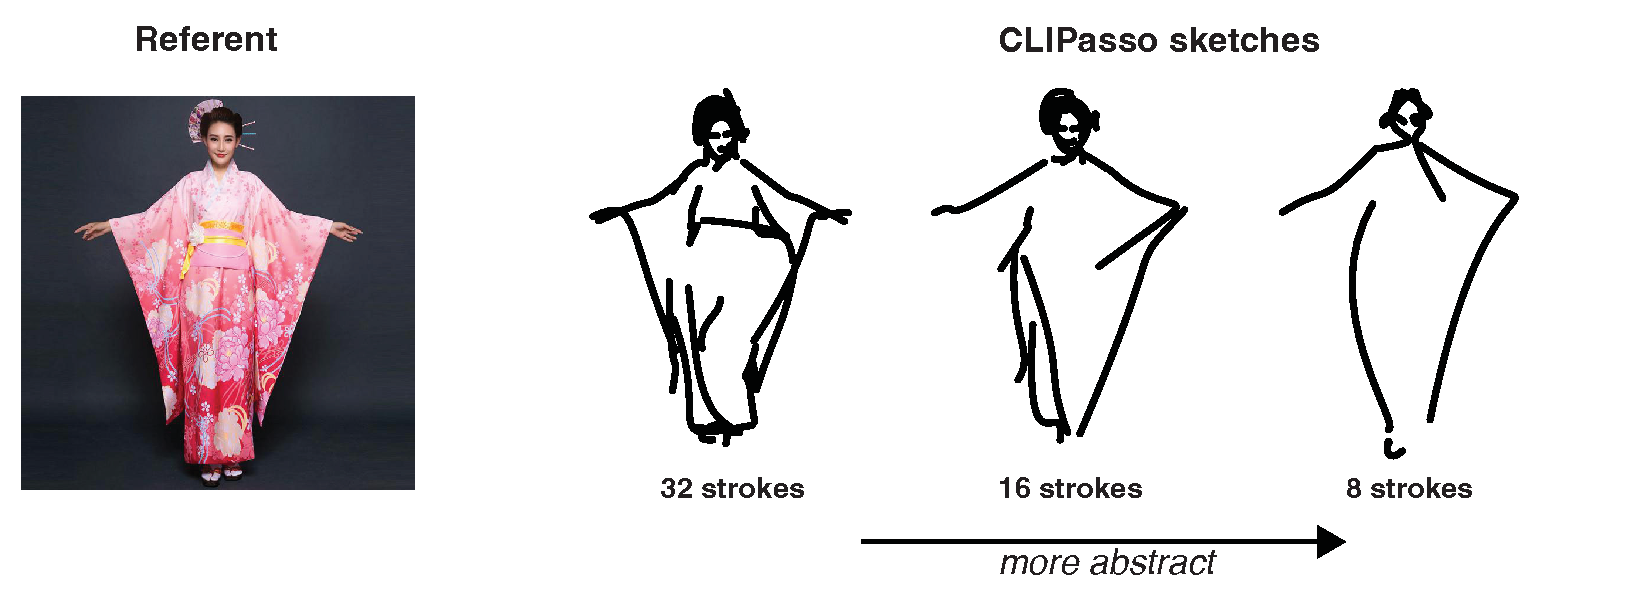
\includegraphics[width=.5\textwidth]{figures/clipasso.pdf}
%     \caption{Machine generated sketches of a photograph at low (32 strokes), medium (16 strokes), and high (8 strokes) levels of abstraction}
%     \label{fig:clipasso_ex}
% \end{figure}

% \begin{figure*}
%     \centering
%     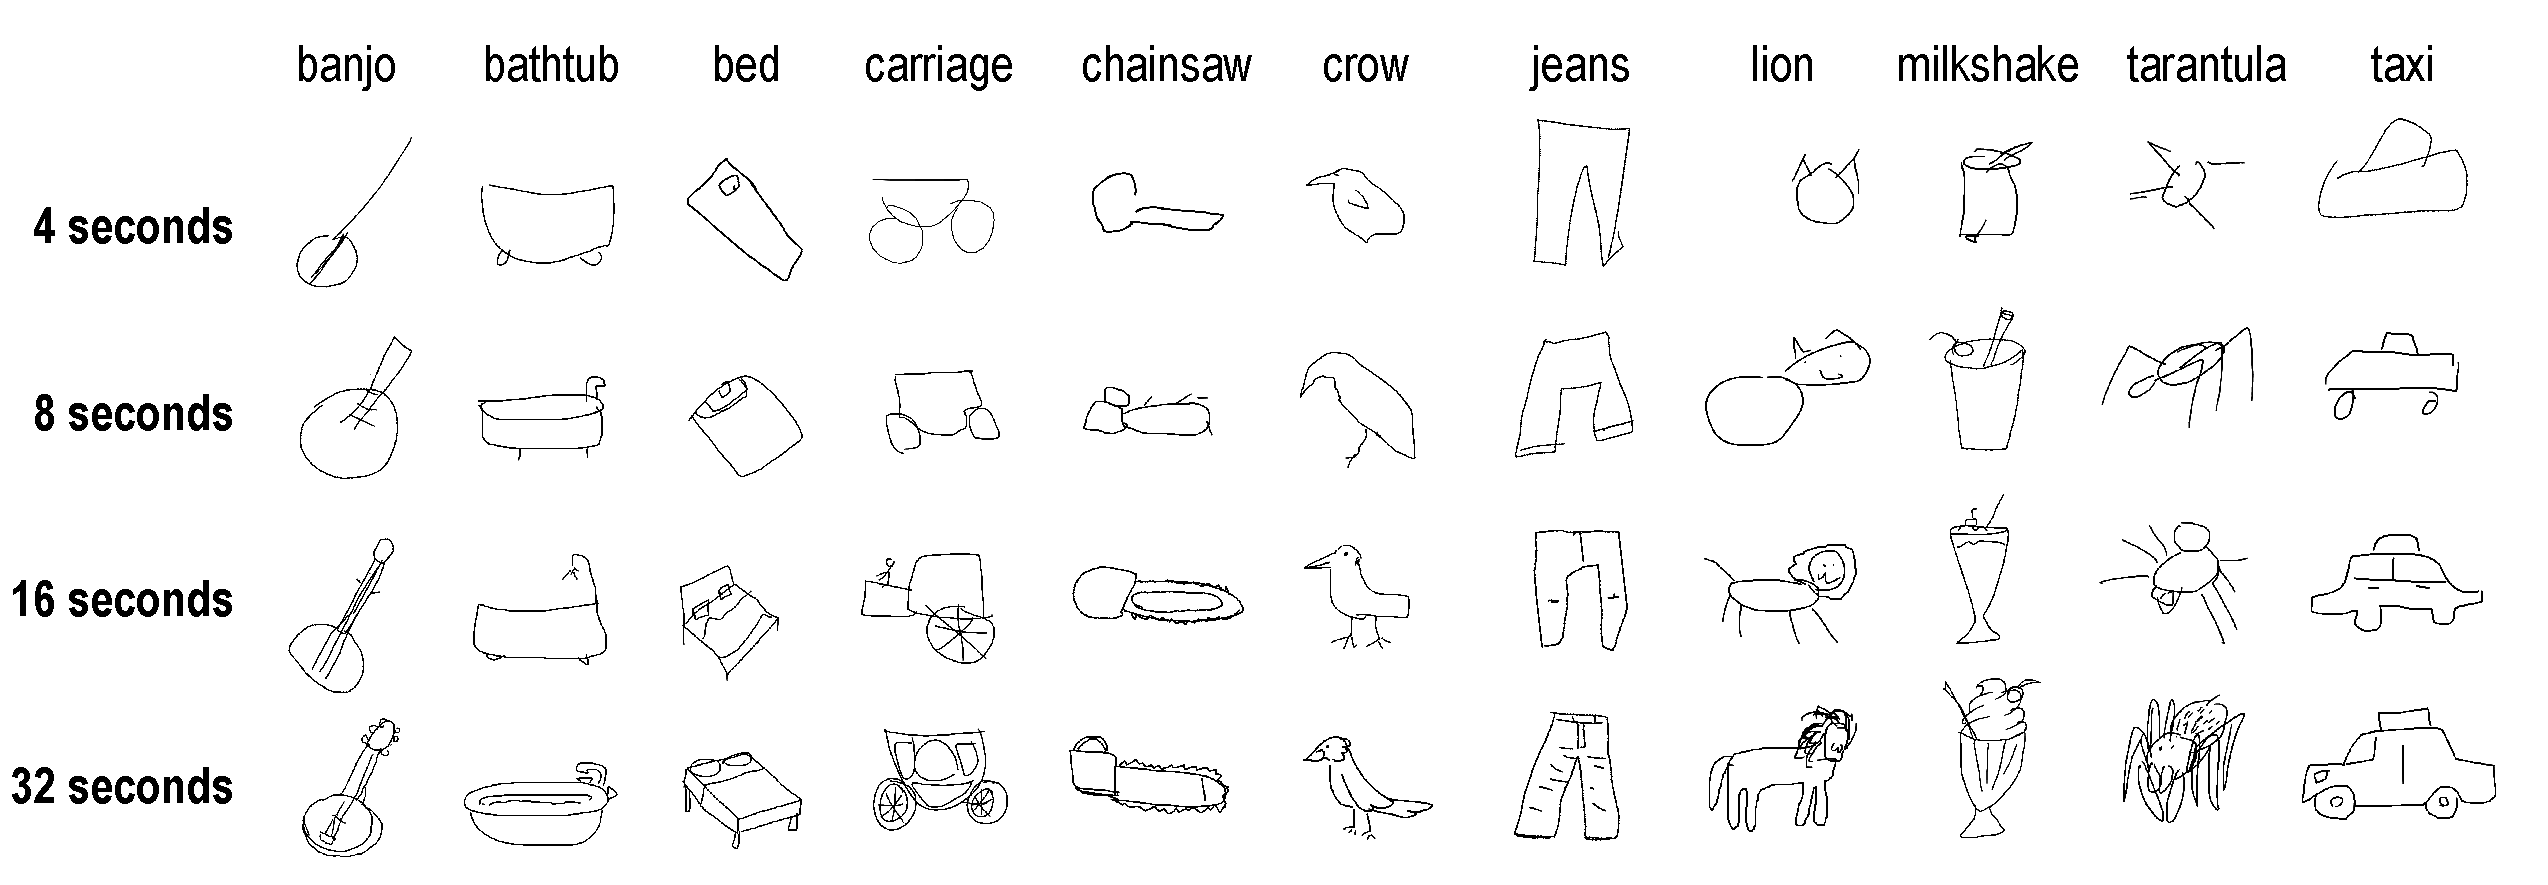
\includegraphics[width= 1\linewidth]{figures/thingsdraw_gallery_alpha.pdf}
%     \caption{Example sketches of objects from the THINGS128 dataset produced under different time limits.}
%     \label{fig:gallery}
% \end{figure*}

% \subsubsection{Results}
% \hh{We collected over 84,000 unique drawings of the THINGS128 dataset. 
% We first tested if there were any meaningful differences between drawings of the same concept across the different timing conditions.
% To accomplish this, we measured the number of unique strokes in a drawing as a metric of the amount of detail included in each drawing and fit a mixed-effects linear regression model with random intercepts for concept type predicting number of strokes as a function of time allotted per drawing showed a significant effect of time.
% We found that drawings produced under the 4s limit contained the least number of average strokes, whereas those produced under the 32s limit contained the most number of average strokes ($\beta=.029$, $t=58.54$, $p<.001$, see Table \ref{tab:strokes} for all four conditions). 
% These results confirm that the time-restriction manipulation elicited meaningful differences in detail across drawing conditions.} 
% % The amount of detailed included in each drawing, measured using the number of unique strokes in a drawing, did increase with increased allowed drawing time with the 4s condition having the fewest strokes and the 32s condition having the most strokes on average. Refer to table \ref{tab:strokes} for information on all 4 conditions.
% % A mixed-effects linear regression model with random intercepts for concept type predicting number of strokes as a function of time allotted per drawing showed a significant effect of time ($\beta=.029$, $t=58.54$, $p<.001$). Thus, our time-restriction manipulation did indeed lead to drawings that varied in level of detail. 
% In order to answer our questions about visual abstraction, we define two complementary metrics to measure the amount of abstraction in a sketch based on its latent representations. 

% \begin{table}[h!]
%     \centering
%     \begin{tabular}{c|l l}
%         Drawing time & $M_{strokes}$ & $SD_{strokes}$\\
%          \toprule
%         4 seconds & 1.61 & 1.49\\
%         8 seconds & 3.49 & 2.43\\
%         16 seconds & 6.39 & 4.27\\
%         32 seconds & 9.90 & 7.11\\
%         \bottomrule 
%     \end{tabular}
%     \caption{Differences in number of strokes used per drawing condition. Longer drawing times resulted in more detailed drawings, but also a greater variance in amount of detail included }
%     \label{tab:strokes}
% \end{table}


\subsection{Formalizing abstraction in vision models}
% \vspace{-1em}
% \begin{figure}[ht!]
%     \centering
%     \includegraphics[width=0.8\linewidth]{figures/VAB_schematic2.pdf}
%      \vspace{-1em}
%     \caption{Calculating metrics: (1) cosine similarities between sketch embeddings and each photo are computed to generate category and exemplar-level similarity distributions; (2) classification accuracy is measured by whether the correct category/exemplar is among the 10 most similar items.
%     % Procedure for computing visual abstraction metrics for a given sketch. Cosine similarities between embeddings for the sketch and each of the 2,048 photographs are computed to generate distributions of category and exemplar level similarities. Classification accuracy is measured by whether the correct exemplar/category is among the 10 most similar items.
%     }
%     \vspace{-1em}
%     \label{fig:_}
%     \vspace{-0.5em}
% \end{figure}
% \vspace{-.8 em}
Which state-of-the-art vision models display human-like understanding of visual concepts at varying levels of abstraction as seen in sketches? 
To make progress towards answering this question, we first curated a set of vision models with varied architectural commitments and training procedures. 
Next, we designed an evaluation protocol such that models' performance could be directly compared to human behavior.

\begin{figure*}
    \centering
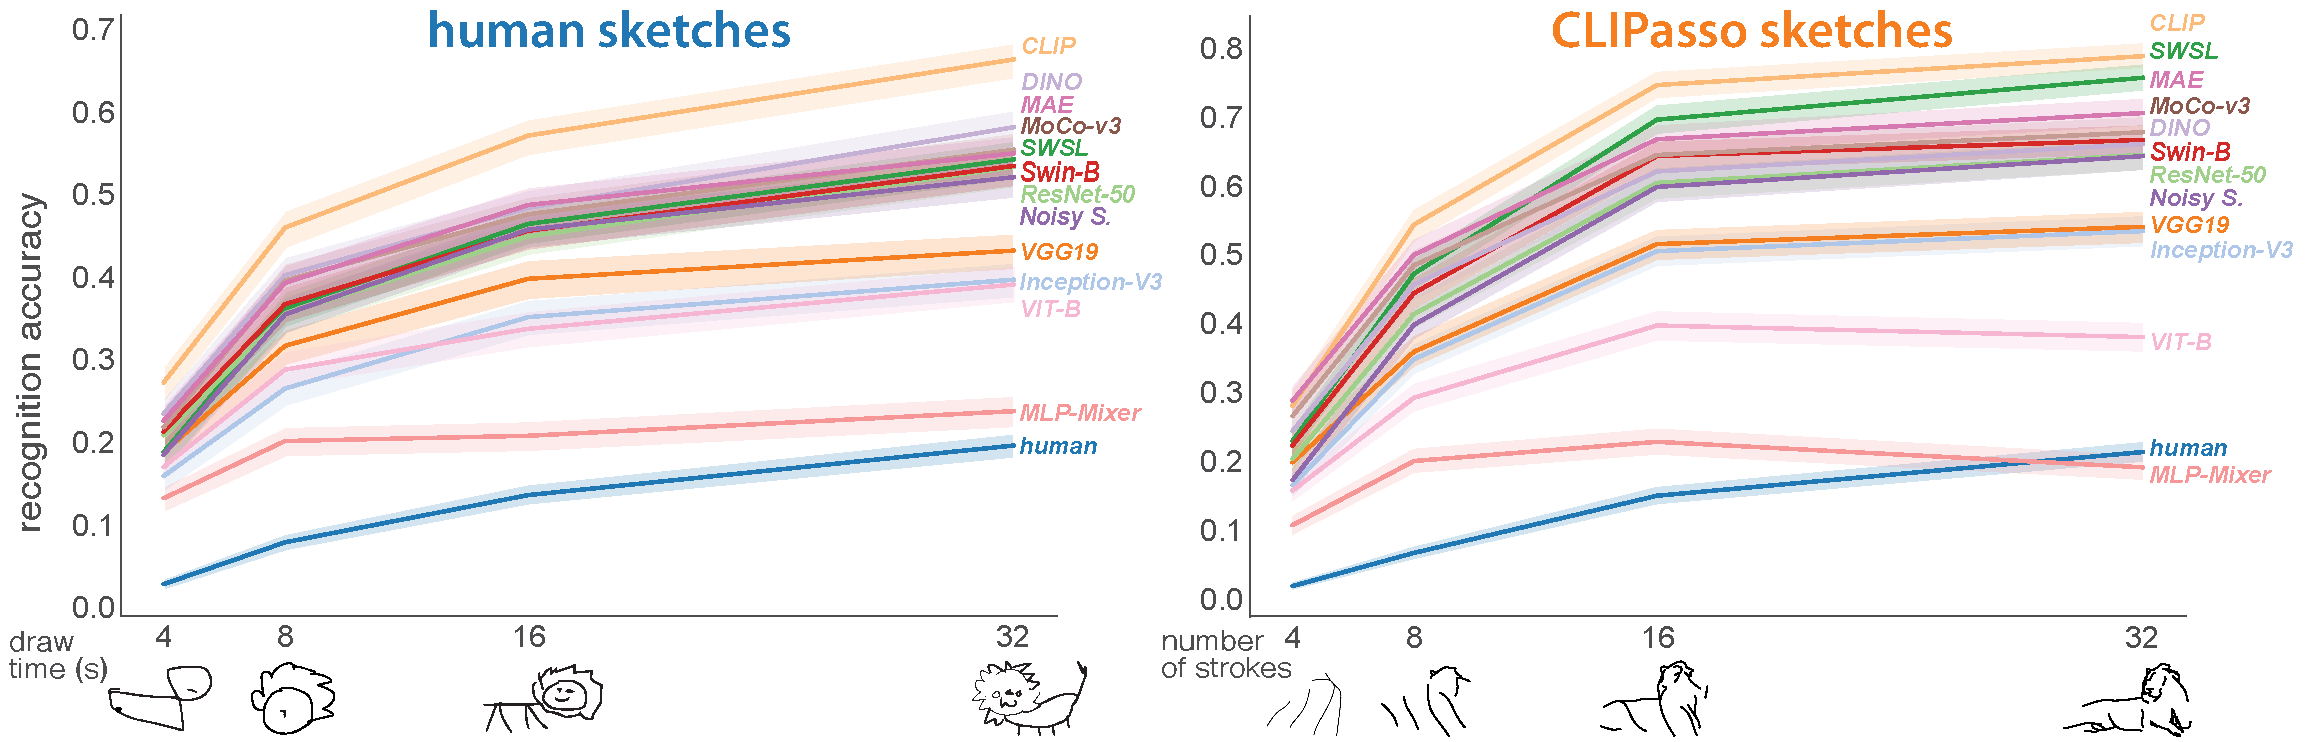
\includegraphics[width=.9\linewidth]{figures/VAB_recog_no_mocov2.pdf}
    \vspace{-1em}
    \caption{Top-1 recognition accuracy by models of human sketches (\textit{left}) and CLIPasso sketches (\textit{right}). Note that human accuracy reflects performance on a 1854-way classification task, rather than on the 128-way task performed by models.}
    \vspace{-1em}
    \label{fig:VAB_recog}
\end{figure*}

\subsubsection{Models} 
We evaluated 12 vision models spanning multiple architectures and training paradigms (see Table \ref{tab:models}), all of which have demonstrated high performance for object recognition on standard datasets like ImageNet \cite{deng2009imagenet}. 
% (supervised learning, self-supervised learning, semi-supervised learning)
% (e.g., convolutional networks (convnets), transformers, multi-layer perceptrons (mlps))
% The models include 3 ImageNet-supervised convnets \cite{deng2009imagenet}, 3 ImageNet-supervised transformers, 4 self-supervised vision models, CLIP, and 2 semi-supervised models 
% Refer to Table \ref{tab:models} for full list of models. 
We performed all downstream computations on latent features extracted from the deepest (non-fully-connected) layers of these models, which amounted to extracting activation patterns at either the model's final convolution or attention layer.
% While these models show high performance for object recognition on standard datasets like Imagenet \cite{deng2009imagenet}, do these gains translate to senstivity to visual abstraction across sketches?

% \begin{table}[htp]
% \centering
% % \vspace{-4mm}
% \resizebox{0.5\textwidth}{!}{%
% \begin{tabular}{l|l|l|l}
% Methods  & Architecture & Training Paradigm & Dataset\\ 
% \hline
% VGG-19~\cite{simonyan2014very} & VGG-19 & supervised & ImageNet\\ 
% Inception-V3~\cite{szegedy2016rethinking} & Inception-V3 & supervised & ImageNet\\
% ResNet-50~\cite{he2016deep} &  ResNet-50  & supervised & ImageNet \\
% ViT-B~\cite{dosovitskiy2020image}  & ViT-B & supervised & ImageNet \\
% Swin-B\cite{liu2021swin} & Swin-B & supervised & ImageNet \\ 
% MLPMixer-B~\cite{tolstikhin2021mlp} & MLPMixer-B & supervised & ImageNet \\ 
% MoCo-v2~\cite{chen2020improved} & ResNet-50 & self-supervised & ImageNet \\ 
% MoCo-v3~\cite{chen2021empirical} & ViT-B & self-supervised & ImageNet \\ 
% DINO~\cite{caron2021emerging} & ViT-B & self-supervised & ImageNet \\ 
% MAE~\cite{he2022masked} & ViT-B & self-supervised & ImageNet \\ 
% CLIP~\cite{radford2021learning} & ViT-B & self-supervised & WebImageText \\ 
% Noisy Student~\cite{xie2020self} & EfficientNet-b4 & semi-supervised & ImageNet + JFT \\
% SWSL~\cite{yalniz2019billion} &  ResNet-50  & semi-supervised & ImageNet + 1B-Targeted \\
% \bottomrule 
% \end{tabular}%
% }
% %\vspace{1mm}
% \caption{The list of models that we evaluated. We show the network architecture, training paradigm, and training dataset of each model.}
% % \vspace{-5mm}
% \label{tab:models}
% \end{table}

\subsubsection{Evaluation Protocol}

% People can recognize both a detailed and sparse sketch of Picasso's bulls as a bull. 
% Are vision models also able to decode the semantic information conveyed in a drawing despite its level of abstraction?
% Here, we outline a protocol for testing this hypothesis.
Due to the varied dimensionality and characteristics of the latent model features (outputs of convolution vs. attention layers vs. linear layers), to fairly assess the semantic information decodable from these features, we fit a series of regularized logistic classifiers predicting the class labels of each sketch from the latent features.
% in order to evaluate each model fairly. 
Classifiers were fit separately to each neural network using 5--fold stratified cross-validation to predict the class label of the sketch. 
For each sketch, when presented in the test fold, we preserved the full vector of class probabilties corresponding to the 1,854 THINGS object classes.\footnote{Human and machine sketches were generated from only 128 classes, thus many class probability values of the full 1,854 THINGS label set were 0.}
% It should be noted that since the THINGS128 dataset, which the classifiers were fit on, only has a subset of the full 1854 labels, many of these logit values were 0.
Next, to compare these model data against human recognition, we leveraged the label data generated from our recognition study to compute the number of times each of the 1,854 labels was assigned to a given sketch.
By summing these label counts across participants and normalizing them, we generated a human recognition ``response'' vector for each sketch, representing a distribution over the 1,854 labels as a measure of its perceived polysemy. 
Importantly, this provided an analogous baseline of comparison to the class probability vectors extracted from the classifiers.
% The spread of these label distributions  for a given sketch can be taken as a measure of its perceived polysemy over the 1854 labels

\begin{table}[hbp!]
\centering
\vspace{-0.5em}
\resizebox{0.5\textwidth}{!}{%
\begin{tabular}{l|l|l}
\textbf{Models}  & \textbf{Architecture} & \textbf{Training Paradigm}\\ 
\hline
\textbf{\textcolor{VGG-19}{VGG-19}}~\cite{simonyan2014very} & VGG-19 & supervised \\ 
\textbf{\textcolor{Inception-V3}{Inception-V3}}~\cite{szegedy2016rethinking} & Inception-V3 & supervised \\
\textbf{\textcolor{ResNet-50}{ResNet-50}}~\cite{he2016deep} &  ResNet-50  & supervised  \\
\textbf{\textcolor{ViT-B}{ViT-B}}~\cite{dosovitskiy2020image}  & ViT-B & supervised\\
\textbf{\textcolor{Swin-B}{Swin-B}}~\cite{liu2021swin} & Swin-B & supervised\\
\textbf{\textcolor{MLPMixer-B}{MLPMixer-B}}~\cite{tolstikhin2021mlp} & MLPMixer-B & supervised\\
% \textbf{\textcolor{MoCo-v2}{MoCo-v2}}~\cite{chen2020improved} & ResNet-50 & self-supervised \\
\textbf{\textcolor{MoCo-v3}{MoCo-v3}}~\cite{chen2021empirical} & ViT-B & self-supervised\\
\textbf{\textcolor{DINO}{DINO}}~\cite{caron2021emerging} & ViT-B & self-supervised\\
\textbf{\textcolor{MAE}{MAE}}~\cite{he2022masked} & ViT-B & self-supervised \\
\textbf{\textcolor{CLIP}{CLIP}}~\cite{radford2021learning} & ViT-B & self-supervised\\
\textbf{\textcolor{Noisy Student}{Noisy Student}}~\cite{xie2020self} & EfficientNet-b4 & semi-supervised\\
\textbf{\textcolor{SWSL}{SWSL}}~\cite{yalniz2019billion} &  ResNet-50  & semi-supervised \\
\bottomrule 
\end{tabular}%
}

% \vspace{-0.5em}
\caption{Evaluated models and their network architecture backbone and training paradigm.}
\vspace{-1em}
\label{tab:models}
\end{table}

\section{Results}
Our final drawing dataset contained over 90,000 unique drawings (90,922 human-produced sketches; 8,191 CLIPasso-generated sketches\footnote{We removed one blank sketch from the CLIPasso dataset.}). 
\subsubsection{Shorter drawing times yield sketches with fewer strokes.}
To validate our manipulation of drawing duration during human sketch production, we counted the number of unique strokes in a drawing as a measure of detail (Fig.~\ref{fig:stroke_counts}) and then fit a mixed-effects linear regression model with random intercepts for category predicting number of strokes as a function of time allotted per drawing.
% showed a significant effect of time.
We found that drawings produced under the 4s limit contained the fewest strokes, whereas those produced under the 32s limit contained the most strokes ($\beta=.29$, $SE=4.95 \times10^{-3}$, $p<.001$).
These results help confirm that the time-restriction manipulation elicited meaningful differences in detail across drawing conditions.
% \vspace{-1em}
\begin{figure*}
    \centering
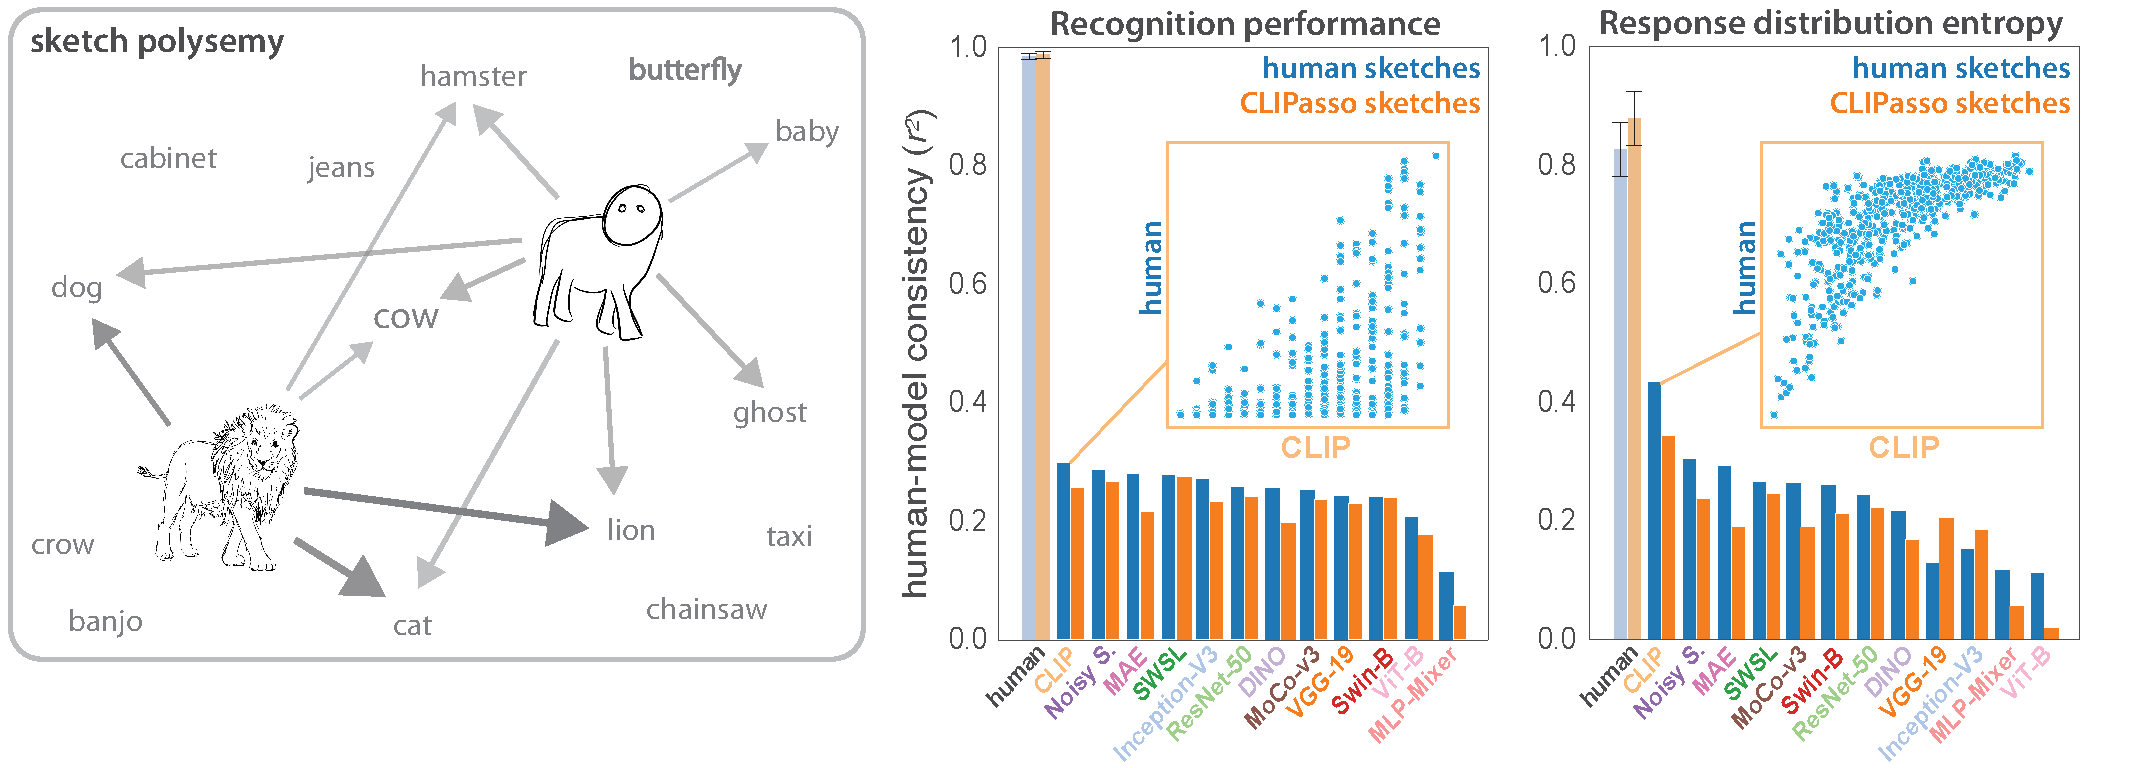
\includegraphics[width=1\linewidth]{figures/VAB_polysemy_no_mocov2.pdf}
    % \vspace{-1em}
    \caption{\textit{Left:} Example of sketch polysemy at different levels of abstraction. \textit{Middle:} Proportion of variance explained in top-1 human recognition accuracy by model top-1 accuracy. \textit{Right:} Proportion of variance explained in human response distribution entropy by model class probability entropy. Inset scatterplots show the distribution of entropy values between human judgements and CLIP.}
    \vspace{-1em}
    \label{fig:VAB_polysemy}
\end{figure*}
% \subsubsection{Varying stroke complexity and draw duration  moderates perceived semantics in sketches for both humans and machines.}

\subsubsection{Production constraints on sketch production impact sketch recognition.}

How well do people and vision models recognize the object concepts represented in sketches? 
And to what extent is the ability to reliably decode the semantic content in a given sketch impacted by the level of abstraction as measured by stroke complexity or time taken to draw it?  
% To answer these questions, we took the top-1 guess from our classifiers and human recognition judgements and looked at whether there was systematic variation in recognition performance as a function of production constraint.
% draw duration (for human sketches) and number of strokes (for machine sketches). 
% As can be seen in figure \ref{fig:recognition_performance}, both humans and models were indeed better at recognizing the object concept in sketches as stroke complexity and draw duration increased.
To evaluate these questions, we fit mixed-effect linear regression models predicting the mean top-1 recognition accuracy in humans and vision models as a function of draw duration for human sketches and number of strokes for CLIPasso sketches. 
We included model-type as an additional fixed effect to test for performance differences between the vision models. 
Finally, we included by-concept intercepts and random slopes for draw duration or number of strokes.
We found a significant effect of draw duration and number of strokes for both human ($\beta_{draw \: duration}=5.66\times10^{-3}$, $SE=5.92\times10^{-4}$, $p<.001$; $\beta_{strokes} = 6.74 \times 10^{-3}$, $SE = 7.17 \times 10^{-3}$, $p<.001$) and model ($\beta_{draw \: duration} = 9.16\times10^{-3}$, $SE= 4.21\times10^{-4}$, $p <.001$; $\beta_{strokes} = 1.21 \times 10^{-2}$, $SE = 3.83 \times 10^{-4}$, $p<.001$) recognition performance, indicating that greater amounts of detail in sketches correspond to higher recognition performance by both humans and vision models (Fig.~\ref{fig:VAB_recog}). 
Additionally, we found an effect of model-type when coding for CLIP as the reference category indicating that not all models are equally performant when discerning the semantic structure in both human ($\chi^2(11)=2712.50$, $p<.001$) and CLIPasso ($\chi^2(11) = 5759.4$, $p<.001$) sketches.


\subsubsection{Vision models vary in their degree of consistency with human recognition performance and response patterns.}
Next, we conducted finer-grain analyses to identify which vision models are most consistent with human recognition performance by: (1) comparing the degree of alignment between model and human recognition \textit{accuracy}; and (2) comparing the degree of alignment between model and human recognition \textit{uncertainty}.
First, we fit mixed-effect linear regression models predicting mean human top-1 accuracy from vision model top-1 accuracy and model-type with by-concept random slopes and intercepts to account for variability within concepts.
We found that model performance was a significant predictor of human recognition performance ( $\beta_{human \; sketches} = 2.96\times10^{-1}$ $SE= 2.36\times 10^{-2}$, $p<.001$; $\beta_{machine \; sketches}= 2.97\times10^{-1}$, $SE = 2.34 \times 10^{-2}$, $p<.001$). 
Furthermore, model comparisons revealed a significant effect of model-type for human ($\chi^2(11)=552.92$, $p<.001$) and machine sketches ($\chi^2(11)=741.51$, $p<.001$), adding additional support that some vision models are more consistent with human recognition performance than others (Fig. \ref{fig:VAB_polysemy}, \textit{middle}).
Specifically, these analyses revealed that CLIP explains the greatest amount of variance in human recognition accuracy, while MLP-Mixer explains little variance.
While there is some discrepancy between which models are more accurate when comparing performance on human sketches vs. CLIPasso sketches, we generally saw that models that have better recognition performance across both datasets (Fig. \ref{fig:VAB_recog}) are also more consistent with human recognition performance. 
% (\ref{fig:recognition_performance}

Second, we computed the entropy of the distributions over object labels for each of the 8,192 sketches across both human sketch and CLIPasso sketch datasets, using the normalized label counts and classifier class probabilities, respectively (Fig.~\ref{fig:VAB_polysemy}, \textit{right}). 
Next, we fit mixed-effect models predicting human response entropy from model class probability entropy and model-type with by-concept random slopes and intercepts for entropy. 
Similar to model comparisons to human recognition accuracy, we found that model entropy significantly predicted human response entropy ($\beta_{human \; sketches}=2.04 \times10^{-1}$, $SE=6.57\times10^{-3}$, $p<.001$; $\beta_{machine \; sketches} = 2.09 \times10^{-1}$, $SE = 7.90 \times10^{-3}$, $p<.001$). 
Additionally, model comparisons revealed a significant effect of model-type for both human ($\chi^2(11) = 1241.30$, $p<.001$) and machine ($\chi^2(11) = 1509.00$, $p<.001$) sketches, although CLIP was found to be the highest performing model for both human and CLIPasso sketches when using this metric.
These evaluations of accuracy and uncertainty reveal that both state-of-the-art model performance and the distributions underlying that performance is predictive of the same constructs for human recognition performance to varying degrees, with some models being more consistent with human behavior than others. 

% Which models are most consistent with human recognition performance? 
% In the previous section, we established that all models were not equal in performance, but are some models systematically better than others in their alignment with human performance? 
% We investigated this question at two levels — we first compared models and humans in the degree to which the aligned in their recognition accuracy and then compared them at a finer level of detail by comparing properties of their response distributions.
% In figure \ref{fig:human_vs_model} (left), it can be seen that CLIP explains the greatest amount of variance in human recognition accuracy, while MocoV2 and the MLP-Mixer explain little variance.
% While there is some discrepancy between which models are the best when looking at comparisons for human vs. machine produced sketches, we generally find that models that have better recognition performance (\ref{fig:recognition_performance} are also more consistent with human responses.

% To account for variability within concepts, we also fit mixed-effect linear regression models predicting mean human top-1 accuracy from model top-1 accuracy and model-type with by-concept random slopes and intercepts.
% Model performance was a significant predictor of human performance ( $\beta_{human \; sketches} = 2.87\times10^{-1}$ $SE= 2.12\times 10^{-2}$, $p<.001$; $\beta_{machine \; sketches}= 2.87\times10^{-1}$, $SE = 2.04 \times 10^{-2}$, $p<.001$) and a model comparison revealed a significant effect of model-type for human ($\chi(12)=631.81$, $p<.001$) and machine sketches ($\chi(12)=822.11$, $p<.001$), supporting the notion that some models are more consistent than others.

% In addition to their top-choice of label, do humans and machines align on their uncertainty as well? 
% That is,  how different are the distributions that underlie their recognition performance?
% To answer this question, we computed the entropy of the distributions over label for each of the 8192 sketches in our recognition dataset. 
% For humans this distribution was computed by adding label counts across participants and normalizing, while for machines this distribution was based on classifier logits. In figure \ref{fig:human_vs_model} (right), we show the amount of variance in human response entropy explained by model-based entropy.

% Here too, we see a similar trend as with recognition accuracy, however with CLIP as the highest performing model for both human and machine sketches.
% Mixed-effect models predicting human response entropy from model logit entropy and model-type with by concept random slopes and intercepts for entropy revealed that model logit entropy significantly predicted human response entropy ($\beta_{human \; sketches}=1.97 \times10^{-1}$, $SE=6.52\times10^{-3}$, $p<.001$; $\beta_{machine \; sketches} = 2.06 \times10^{-1}$, $SE = 7.66 \times10^{-3}$, $p<.001$). 
% Similar to recognition accuracy, model comparisons revealed a significant effect of model-type for both human ($\chi^2 = 1475.20$, $p<.001$) and machine ($\chi^2 = 1746.30$, $p<.001$) sketches  .

% \subsubsection{Models are consistent in their representations of sketches made under different constraints}

% While there is consistency within model architectures in the degree to which they are sensitive to semantic information, is there a meaningful effect of constraint level (time or number of strokes) on performance across all models? 
%  Are models' understanding of sketches made under lighter constraints—more drawing time, greater number of strokes—more varied relative to sketches made under tighter constraints? If different models are sensitive to different visual features, which might arise with more detailed drawings, one might expect to see a negative correlation between constraint level and performance consistency.

% To test this hypothesis, we once again constructed model-model performance similarity matrices at both the exemplar and category level. 
% We computed the average similarity within each constraint condition (4 for human drawings, 3 for machine drawings) and estimated the slope of the relationship between these 2 factors. 
% To test the statistical significance of the slope we permuted the matrix-generating dataset 10000 times and constructed a null-distribution of similarity-by-constraint slopes. Under this distribution the observed true slopes were not significant at either the exemplar ($p_{human} = .86$,$ p_{machine}  = .81$) or category level ($p_{human}  = .82$, $p_{machine} = .99$). 
% Thus, current vision models are consistent in their sensitivities to semantic information across different abstraction conditions


% Thus, our series of tests reveal that both model performance and the distributions underlying that performance can predict those same constructs for human behavior to varying degrees, with some models being more consistent with human behavior than others. 
% \vspace{-.5em}
\subsubsection{Sketch recognition behavior is generally consistent across vision models.} % Representations of semantic uncertainty are generally undistinguished across models.

To what degree are state-of-the-art vision models consistent in their sensitivity to the semantic information conveyed by sketches containing varying amounts of detail?
% Some models are more consistent with human behavior than others in terms of their sensitivity to the semantic information conveyed by sketches at varying levels of detail.
% But are different models consistent within themselves in how they represent the uncertainty over object labels across sketches in a way that distinguishes them from other models?
To evaluate this question, we looked at how consistent different models were in their patterns of average uncertainty over the sketches belonging to each of the 128 object classes and whether this consistency changed as function of stroke count or draw duration.
% how consistent the response distributions over the THINGS128 object labels were across models at different levels of stroke complexity.
% we measured if the distributions of object label entropy values produced by different production constraints were more similar \textit{within} a model than across models.
For each model, we first computed 128-dimensional \textit{entropy vectors} to capture the uncertainty expressed by the model for each of the object classes. 
Each resulting entry in this vector was the average response distribution entropy across sketches for one of the classes.
If two models shared similar entropy vectors, it would indicate similar patterns of uncertainty across sketches of each class.
To measure how consistent models are across each production constraint level, we computed separate entropy vectors for each model at each production constraint level for both sketch datasets (number of strokes for CLIPasso sketches and draw duration for human sketches).
% We first computed 128-dimensional object label entropy vectors for each model at each production constraint level, by computing the average model logit entropy for all sketches of both human sketch and CLIPasso sketch datasets.

% Next, these vectors were used to construct similarity matrices where each cell corresponded to the Pearson correlation between each vector pair.

% For each dataset and for each model, we computed the ratio between the average of within-model distances and average of between-model distances, where larger values closer to 1 would indicate stronger model internal consistency.
% To evaluate how reliably different these ratios were from chance, we permuted each row of the matrix generating dataset in order to disrupt the model-based grouping and computed the within-model vs. between-model distance ratio 10,000 times to generate a null distribution. 
% After applying the Bonferroni correction to correct for multiple tests (one for each model), we tested our observed ratio against this hull distribution and found that only ``mocoV2's'' representations were significantly more consistent within itself, relative to other models for both human and CLIPasso sketches ($p<.05$). 
% These results suggest that state-of-the-art vision models are generally consistent with each other when making object classifications of sketches at different levels of abstraction. 

\begin{figure}[h!]
    \centering
    % \vspace{-1em}
    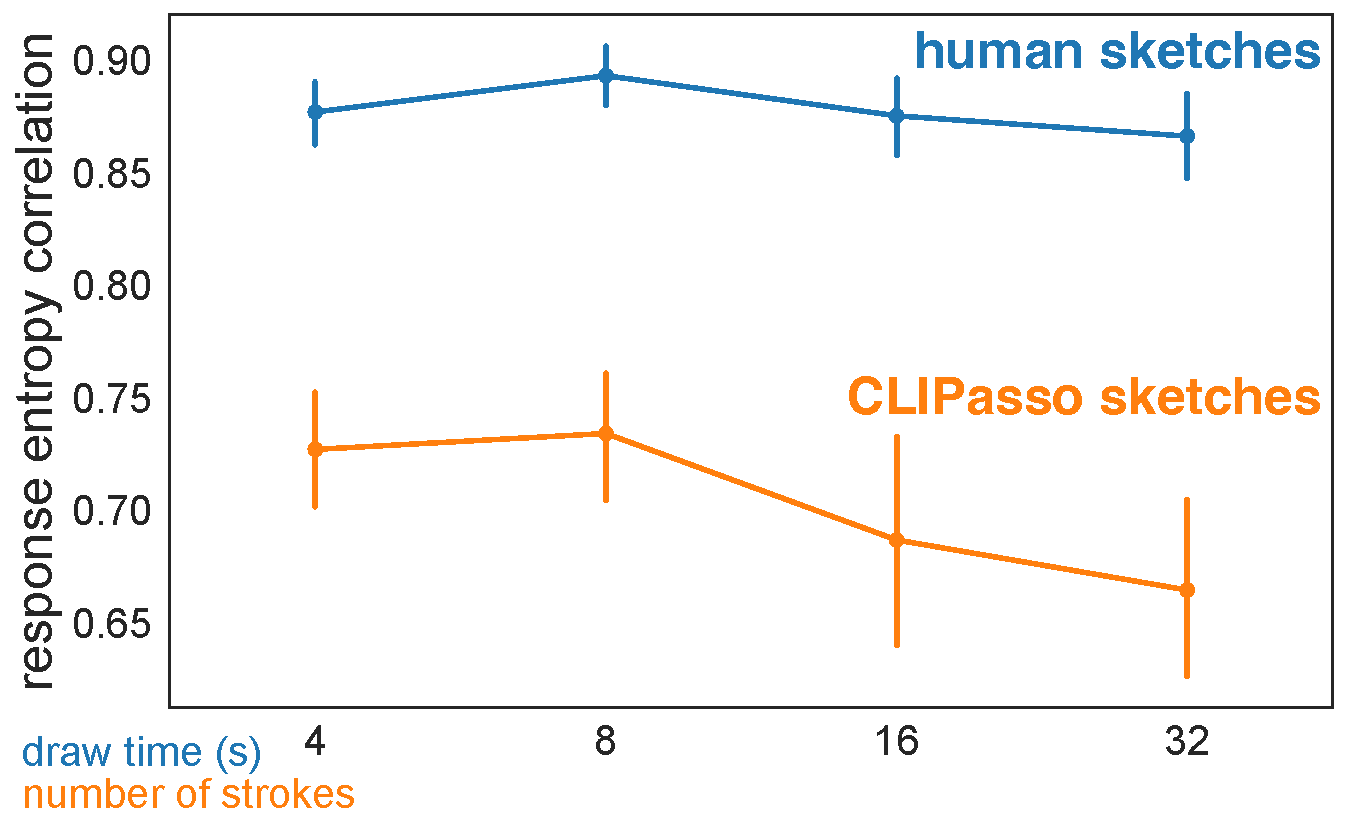
\includegraphics[width=.9\linewidth]
    {figures/VAB_H_cor_vs_complexity.pdf}
    \vspace{-1em}
    \caption{Mean correlation between response entropy vectors across models at different abstraction levels.}
    \label{fig:VAB_H_cor_vs_complexity}
    \vspace{-1em}
\end{figure}
We found a high average correlation between entropy vectors across models for each production constraint level and for both sketches generated by human sketchers and CLIPasso (Fig.~\ref{fig:VAB_H_cor_vs_complexity}), suggesting that all the models appeared to represent semantic uncertainty in a generally similar manner when classifying sketches of different object classes. 
Additionally, we conducted model comparisons between two linear regression models predicting response correlation, one with a factor for draw duration and one without. 
We found that a factor for draw duration did not explain significantly unique variance in the model relative to the intercept-only model ($F(260,3) = 1.78$, $p = .15$). 
These results indicate that models were equally consistent in their uncertainty when generating classifications of human sketches of different object classes. 
For sketches generated using CLIPasso, we also compared an intercept-only model to a model with a factor for number of strokes and found a significant effect of number of strokes ($F (3,260) = 3.19$, $p < .05$).
Thus, for machine generated sketches, there did appear to be an effect of stroke number on the consistency between models in their expressed semantic uncertainty with models being less consistent in their classifications of sketches with more strokes. 
Taken together, these results suggest that sketch recognition behavior is generally consistent across these 12 state-of-the-art vision models, particularly for sketches produced by humans and despite being drawn at varying levels of detail. 

% in their expressed uncertainty over different classes with more detailed sketches leading models to be less consistent

% Across levels of detail, models were equally consistent in their uncertainty over the different classes for human sketches. 
% This notion was supported by a model comparison between two linear regression models predicting response correlation, one with a factor for draw duration and one without. 
% The factor for draw duration did not explain significantly unique variance in the model relative to the intercept-only model ($F(260,3) = 1.78$, $p = .15$).
% For CLIPasso sketches, there did appear to be an effect of number of strokes on the consistency between models in their expressed uncertainty over different classes with more detailed sketches leading models to be less consistent.
% Similar to the human sketches, we compared an intercept-only model to a model with a factor for number of strokes and did find a significant effect of number of strokes ($F (3,260) = 3.19$, $p < .05$).
\vspace{-.5em}
\section{Discussion}

There has been incredible progress in the development of high performing vision models over the past several years--and recently, reaching enough variation in model architecture and training to prime cognitive psychology research with the opportunity to begin explore the extent to which specific models have achieved human-like understanding of abstract symbolic representations, like sketches.
To evaluate this expansive range of state-of-the-art vision models and their ability to extract meaning from sketch representations, we introduce a new large-scale drawing dataset of over 90K sketches based on 2,048 real-world objects spanning 128 diverse concept categories.
Our dataset combines both human-made and AI-generated sketches produced under varying production constraints (limitations in drawing duration for human sketchers, and limitations in number of strokes for CLIPasso \cite{vinker2022clipasso}). 
By systematically varying the level of abstraction produced by these different production constraints, our dataset provides a rich testbed to investigate human and machine visual understanding of human and machine sketches. 

% human sketch production behavior by comparing AI sketch generation behavior and human visual recognition performance compared to classification performance by 12 different state-of-the-art vision models, varying in architectures and training techniques. 
In an era where it is becoming increasingly difficult to adjudicate between state-of-the-art vision models in terms of their relevance to human cognition, our dataset provides a novel substrate to tease apart which models are more human-like than others \cite{golan2020controversial}.
We provide initial benchmarking of a representative set of vision models spanning architectures and training techniques against human generated soft-label distributions for a representative set of sketches from both datasets. 
Across a battery of model evaluations, we broadly find that the models that we investigated are sensitive to the variation in the semantic information produced by different production constraints and that some models, like CLIP, are more consistent with human recognition of sketches than others, like MLP-Mixer. 
We also found that models generally agree in their expressed uncertainty over object classes when recognizing sketches and that this uncertainty remains largely consistent across varying levels of abstraction and detail, but with models being less consistent across abstraction levels over their uncertainty in machine generated sketches.
This points to an intriguing yet critical gap in the fidelity of sketch production algorithms to human sketch behavior, and we hope results such as ours will help open avenues for closing this gap in human-machine sketch production.

% However, we also found that while some models outperform others, they are difficult to distinguish in terms of how they express uncertainty over class labels across concepts. 
% While models are equally consistent in their uncertainty for human sketches at varying level of detail, this uncertainty is less consistent for more detailed machine-generated sketches.

% These findings generally resonate with \citeauthor{bansal2021revisiting}'s (2021) ``Anna Karenina Conjecture'', which posits that higher performing models ``hang together'' and subsequently have more similar internal representations.
% We explore methods to arrive at fine-grained metrics of performance, which might help distinguish between models. 
% Namely we observe that analyzing the distribution over object labels causes certain models to appear more aligned with human behavior (such as CLIP) and causes other models (such as mocoV2) to appear less aligned.
% Here we consider an aspect of visual cognition as fundamental as it is evasive to formalize — visual abstraction — and evaluate models on their sensitivity to this construct. 

Within our present work, we offer object concept classification as an initial benchmarking protocol to evaluate different models.
However, we predict future work will seek to benchmark a wider variety of models including those inspired by cognitive neuroscience \cite{chen2022unsupervised, zhuang2021unsupervised,kubilius2019brain} and will seek to build more robust metrics of abstraction beyond those tied to classification-based accuracy.

Our work complements ongoing efforts to understand how different components of current AI vision models give rise to their classification behavior \cite{hermann2020shapes, nguyen2020wide,schott2021visual,chen2021intriguing} and where limitations might arise in mapping model performance to human cognition \cite{ zhou2019humans,bowers2022deep, mahowald2023dissociating}. 
In the long run, progress along these research fronts may shed light upon the computational basis of humans' ability to produce highly abstract but nonetheless meaningful representations, as well as invented symbolic systems for encoding abstract knowledge in pictorial form.
% \cite{schmandt2010writing, chrisomalis2020reckonings}.


% \cite{hawkins2021visual, garrod2007foundations}
\vspace{-.5em}
\section{Acknowledgments}

Many thanks to the members of the Cognitive Tools Lab at UC San Diego for their helpful feedback and support. 
This work was supported by an NSF CAREER Award \#2047191 to J.E.F..
J.E.F is additionally supported by an ONR Science of Autonomy award and a Stanford Hoffman-Yee grant.


\vspace{1em}
\fbox{\parbox[b][][c]{.4\textwidth}{\centering {All code and materials available at: \\
\href{https://github.com/cogtoolslab/visual_abstractions_benchmarking_public2023/}{\url{https://github.com/cogtoolslab/visual_abstractions_benchmarking_public2023/}}
}}}


\bibliographystyle{apacite}

\setlength{\bibleftmargin}{.125in}
\setlength{\bibindent}{-\bibleftmargin}
% \newpage
\bibliography{references}




\end{document}


